%iffalse%\let\negmedspace\undefined
\let\negthickspace\undefined
\documentclass[journal,12pt,onecolumn]{IEEEtran}
\usepackage{cite}
\usepackage{amsmath,amssymb,amsfonts,amsthm}
\usepackage{algorithmic}
\usepackage{graphicx}
\usepackage{textcomp}
\usepackage{xcolor}
\usepackage{caption}
\usepackage{txfonts}
\usepackage{listings}
\usepackage{enumitem}
\usepackage{mathtools}
\usepackage{gensymb}
\usepackage{comment}
\usepackage{tfrupee}
\usepackage[breaklinks=true]{hyperref}
\usepackage{tkz-euclide} 
\usepackage{listings}
\usepackage{gvv}                                        
%\def\inputGnumericTable{}                                 
\usepackage[latin1]{inputenc}   
\usepackage{xparse}
\usepackage{color}                                            
\usepackage{array}                                            
\usepackage{longtable}                                       
\usepackage{calc}                                             
\usepackage{multirow}
\usepackage{multicol}
\usepackage{hhline}                                           
\usepackage{ifthen}                                           
\usepackage{lscape}
\usepackage{tabularx}
\usepackage{array}
\usepackage{float}
\newtheorem{theorem}{Theorem}[section]
\newtheorem{problem}{Problem}
\newtheorem{proposition}{Proposition}[section]
\newtheorem{lemma}{Lemma}[section]
\newtheorem{corollary}[theorem]{Corollary}
\newtheorem{example}{Example}[section]
\newtheorem{definition}[problem]{Definition}
\newcommand{\BEQA}{\begin{eqnarray}}
\newcommand{\EEQA}{\end{eqnarray}}
\usepackage{float}
%\newcommand{\define}{\stackrel{\triangle}{=}}
\theoremstyle{remark}
\usepackage{ circuitikz }
%\newtheorem{rem}{Remark}
% Marks the beginning of the document this one
\title{ AE : AEROSPACE ENGINEERING}
\author{EE25BTECH11018-Darisy Sreetej}
\begin{document}
\maketitle

\section{General Aptitude (GA)}
\textbf{Q.1 - Q.5 Carry ONE mark Each}

\begin{enumerate}
    \item   
If $\rightarrow$ denotes increasing order of intensity, then the meaning of the words  
[dry $\rightarrow$ arid $\rightarrow$ parched ]is analogous to [diet $\rightarrow$ fast $\rightarrow$ \dots].  

Which one of the given options is appropriate to fill the blank?  
\begin{enumerate}
\begin{multicols}{4}
\item starve
\item reject
\item feast
\item deny
\end{multicols}
\end{enumerate}

\item 
If two distinct non-zero real variables $x$ and $y$ are such that $(x+y)$ is proportional to $(x-y)$ then the value of $\dfrac{x}{y}$  
\begin{enumerate}
\begin{multicols}{2}
\item depends on $xy$
\item depends only on $x$ and not on $y$
\item depends only on $y$ and not on $x$
\item is a constant
\end{multicols}
\end{enumerate}

\item
Consider the following sample of numbers: $9, 18, 11, 14, 15, 17, 10, 69, 11, 13$ . The median of the sample is  
\begin{enumerate}
\begin{multicols}{4}
\item 13.5
\item 14
\item 11
\item 18.7
\end{multicols}
\end{enumerate}
  
\item 
The number of coins of $ \rupee 1  $, $\rupee 5$, and $\rupee 10$ denominations that a person has are in the ratio $5:3:13$.  
Of the total amount, the percentage of money in $\rupee 5$ coins is  
\begin{enumerate}
\begin{multicols}{4}
\item 21\%
\item $14\dfrac{2}{7}$\%
\item 10\%
\item 30\%
\end{multicols}
\end{enumerate}


\item 
For positive non-zero real variables $p$ and $q$, if $\log (p^2 + q^2) = \log p + \log q + 2 \log 3$ ,then the value of $\dfrac{p^4+q^4}{p^2 q^2}$ is  
\begin{enumerate}
\begin{multicols}{4}
\item 79
\item 81
\item 9
\item 83
\end{multicols}
\end{enumerate}

\textbf{Q.6 - Q.10 Carry TWO mark Each}

\item  In the given text, the blanks are numbered (i)-(iv). Select the best match for all the blanks.  Steve was advised to keep his head \dots(i)\dots before heading \dots(ii)\dots to bat; for, while he had a head \dots(iii)\dots batting, he could only do so with a cool head \dots(iv)\dots his shoulders.  
\begin{enumerate}
\begin{multicols}{2}
\item (i) down  (ii) down  (iii) on  (iv) for
\item (i) on  (ii) down  (iii) for  (iv) on
\item (i) down  (ii) out  (iii) for  (iv) on
\item (i) on  (ii) out  (iii) on  (iv) for
\end{multicols}
\end{enumerate}


\item 
A rectangular paper sheet of dimensions $54 \,\text{cm} \times 4 \,\text{cm}$ is taken.  
The two longer edges of the sheet are joined together to create a cylindrical tube.  
A cube whose surface area is equal to the area of the sheet is also taken.  
Then, the ratio of the volume of the cylindrical tube to the volume of the cube is  
\begin{enumerate}
\begin{multicols}{4}
\item $\dfrac{1}{\pi}$
\item $\dfrac{2}{\pi}$
\item $\dfrac{3}{\pi}$
\item $\dfrac{4}{\pi}$
\end{multicols}
\end{enumerate}

\item 
The pie chart presents the percentage contribution of different macronutrients to a
typical 2,000 kcal diet of a person. 
\begin{figure}[H]
    \centering
    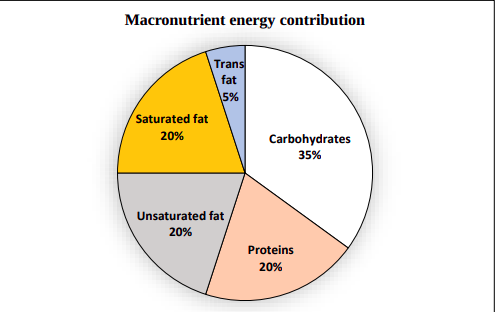
\includegraphics[width=0.5\columnwidth]{figs/Screenshot from 2025-08-23 14-43-47.png}
    \caption{Caption}
    \label{fig:placeholder}
\end{figure}
The typical energy density (kcal/g) of these macronutrients is given in the table. 

\begin{center}
\begin{tabular}{ll}
    \textbf{Group I} & \textbf{Group II} \\
    P. Ferrite & 1. Hexagonal Close Packed (HCP) \\
    Q. Austenite & 2. Body Centered Cubic (BCC) \\
    R. Martensite & 3. Body Centered Tetragonal (BCT) \\
    & 4. Face Centered Cubic (FCC)
\end{tabular}
\end{center}

The total fat (all three types), in grams, this person consumes is
\begin{enumerate}
\begin{multicols}{4}
\item $44.4$
\item $77.8$
\item $100$
\item $3600$
\end{multicols}
\end{enumerate}

  \item 
A rectangular paper of $20 \,\text{cm} \times 8 \,\text{cm}$ is folded 3 times.  
Each fold is made along the line of symmetry, which is perpendicular to its long edge.  
The perimeter of the final folded sheet (in cm) is  
\begin{enumerate}
\begin{multicols}{4}
\item 18
\item 24
\item 20
\item 21
\end{multicols}
\end{enumerate}


\item 
The least number of squares to be added in the figure to make AB a line of symmetry is  

\begin{figure}[H]
    \centering
    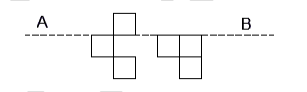
\includegraphics[width=0.5\columnwidth]{figs/Screenshot from 2025-08-23 15-02-24.png}
    \caption{Caption}
    \label{fig:placeholder}
\end{figure}

\begin{enumerate}
\begin{multicols}{4}
\item 6
\item 4
\item 5
\item 7
\end{multicols}
\end{enumerate}

\newpage

\section{Aerospace Engineering (AE)}
\textbf{Q.11 - Q.35 Carry ONE mark Each}

\item 
The following system of linear equations  

$7x - 3y + z = 0$  
$3x - y + z = 0$  
$x - y - z = 0$  

has:  
\begin{enumerate}
\begin{multicols}{2}
\item infinitely many solutions
\item a unique solution
\item no solution
\item three solutions
\end{multicols}
\end{enumerate}
\hfill(GATE AE 2024)

\item 
The acceleration of a body travelling in a straight line is given by  
$a = -C_1 - C_2 v^2$  
where $v$ is the velocity, and $C_1, C_2$ are positive constants. Starting with an initial positive velocity $v_0$, the distance travelled by the body before coming to rest for the first time is:  


\begin{enumerate}
\begin{multicols}{2}
\item $\dfrac{1}{2C_2}\ln \left(1+\dfrac{C_2}{C_1}v_0^2\right)$
\item $\dfrac{1}{2C_2}\ln \left(1-\dfrac{C_2}{C_1}v_0^2\right)$
\item $\dfrac{1}{2C_2}\ln (C_1 + C_2 v_0^2)$
\item $\dfrac{1}{2C_2}\ln (1 + C_2 v_0^2)$
\end{multicols}
\end{enumerate}
\hfill(GATE AE 2024)

\item
The three-dimensional stress-strain relationship for an isotropic material is given as  

$
\myvec{
\sigma_{xx} \\
\sigma_{yy} \\
\sigma_{zz} \\
\tau_{yz} \\
\tau_{xz} \\
\tau_{xy}
}
=
\myvec{
P & Q & Q & 0 & 0 & 0 \\
Q & P & Q & 0 & 0 & 0 \\
Q & Q & P & 0 & 0 & 0 \\
0 & 0 & 0 & R & 0 & 0 \\
0 & 0 & 0 & 0 & R & 0 \\
0 & 0 & 0 & 0 & 0 & R
}
\myvec{
\varepsilon_{xx} \\
\varepsilon_{yy} \\
\varepsilon_{zz} \\
\gamma_{yz} \\
\gamma_{xz} \\
\gamma_{xy}
}
$

where $P, Q, R$ are the three elastic constants. Which one of the following options is correct?  


\begin{enumerate}
\begin{multicols}{2}
\item $R = \dfrac{P - Q}{2}$
\item $R = \dfrac{Q - P}{2}$
\item $Q = \dfrac{P - R}{2}$
\item $Q = \dfrac{R - P}{2}$
\end{multicols}
\end{enumerate}
\hfill(GATE AE 2024)

\item 
Consider the free vibration responses P, Q, R and S (shown in the figure) of a single degree of freedom spring-mass-damper system with the same initial conditions. For the different damping cases listed below, which one of the following options is correct?  

1. Overdamped  
2. Underdamped  
3. Critically damped  
4. Undamped  

\begin{figure}[H]
    \centering
    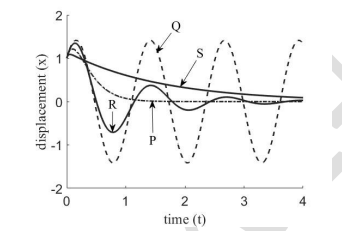
\includegraphics[width=0.5\columnwidth]{figs/Screenshot from 2025-08-23 15-17-56.png}
    \caption{Caption}
    \label{fig:placeholder}
\end{figure}

\begin{enumerate}
\begin{multicols}{2}
\item P - 1, Q - 4, R - 2, S - 3
\item P - 1, Q - 2, R - 4, S - 3
\item P - 3, Q - 4, R - 2, S - 1
\item P - 3, Q - 2, R - 4, S - 1
\end{multicols}
\end{enumerate}
\hfill(GATE AE 2024)

\item 
For a single degree of freedom spring-mass-damper system subjected to harmonic forcing, the part of the motion (response) that decays due to damping is known as:  
\begin{enumerate}
\begin{multicols}{2}
\item transient response
\item steady-state response
\item harmonic response
\item non-transient response
\end{multicols}
\end{enumerate}
\hfill(GATE AE 2024)


\item For an ideal gas, the specific heat at constant pressure is $1147 \ \text{J/kgK}$ and the ratio of specific heats is equal to $1.33$. What is the value of the gas constant for this gas in J/kgK?  
\begin{enumerate}
\begin{multicols}{4}
\item 284.6
\item 1005
\item 862.4
\item 8314
\end{multicols}
\end{enumerate}
\hfill(GATE AE 2024)

\item A surrogate liquid hydrocarbon fuel, approximated as $C_{10}H_{12}$, is being burned in a 
land-based gas turbine combustor with dry air ($79\% \ N_2$ and $21\% \ O_2$ by volume).  
How many moles of dry air are required for the stoichiometric combustion of the surrogate 
fuel with dry air at atmospheric temperature and pressure?  

\begin{enumerate}
\begin{multicols}{4}
\item 61.9
\item 30.95
\item 13
\item 10
\end{multicols}
\end{enumerate}
\hfill(GATE AE 2024)

\item In the figure shown below, various thermodynamics processes for an ideal gas are represented. Match each curve with the process that it best represents.  

\begin{figure}[H]
    \centering
    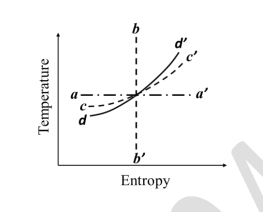
\includegraphics[width=0.5\columnwidth]{figs/Screenshot from 2025-08-23 15-28-11.png}
    \caption{Caption}
    \label{fig:placeholder}
\end{figure}

\begin{enumerate}
\item aa' - Isentropic; bb' - Isothermal; cc' - Isobaric; dd' - Isochoric
\item aa' -  Isothermal; bb' - Isentropic; cc' - Isochoric; dd' - Isobaric
\item aa' - Isothermal; bb' - Isentropic; cc' - Isobaric; dd' - Isochoric
\item aa' - Isothermal; bb' - Isobaric; cc' - Isentropic; dd' - Isochoric
\end{enumerate}
\hfill(GATE AE 2024)

\item In an airbreathing gas turbine engine, the combustor inlet temperature is $600 \ \text{K}$. The heating value of the fuel is $43.4 \times 10^6 \ \text{J/kg}$. Assume $C_p = 1100 \ \text{J/kgK}$ for air and burned gases, and fuel-air ratio $f \ll 1.0$. Neglect kinetic energy at the inlet and exit of the combustor and assume $100\%$ burner efficiency. What is the fuel-air ratio required to achieve $1300 \ \text{K}$ temperature at the combustor exit?  

\begin{enumerate}
\begin{multicols}{4}
\item 0.0177
\item 0.0215
\item 0.0127
\item 0.0277
\end{multicols}
\end{enumerate}
\hfill(GATE AE 2024)

\item Which one of the following figures represents the drag polar of a general aviation aircraft?  

\begin{enumerate}
\item 

\begin{figure}[H]
    \centering
    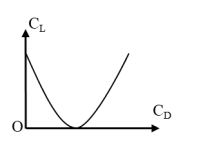
\includegraphics[width=0.5\columnwidth]{figs/Screenshot from 2025-08-23 15-41-27.png}
    \caption{Caption}
    \label{fig:placeholder}
\end{figure}

\item 

\begin{figure}[H]
    \centering
    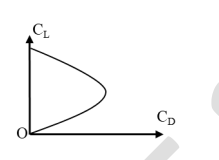
\includegraphics[width=0.5\columnwidth]{figs/Screenshot from 2025-08-23 15-42-43.png}
    \caption{Caption}
    \label{fig:placeholder}
\end{figure}

\item 

\begin{figure}[H]
    \centering
    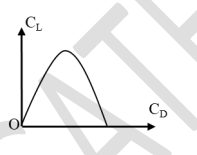
\includegraphics[width=0.5\columnwidth]{figs/Screenshot from 2025-08-23 15-43-49.png}
    \caption{Caption}
    \label{fig:placeholder}
\end{figure}

\item 

\begin{figure}[H]
    \centering
    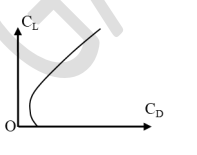
\includegraphics[width=0.5\columnwidth]{figs/Screenshot from 2025-08-23 15-44-38.png}
    \caption{Caption}
    \label{fig:placeholder}
\end{figure}

\end{enumerate}
\hfill(GATE AE 2024)

\item In the context of steady, inviscid, incompressible flows, consider the superposition 
of a uniform flow with speed $U$ along the positive x-axis (from left to right), and a source 
of strength $\Lambda$ located at the origin. Which one of the following statements is NOT true 
regarding the location of the stagnation point of the resulting flow?  

\begin{enumerate}
\item It is located to the left of the origin
\item It moves closer to the origin for increasing $\Lambda$, while $U$ is held constant
\item It moves closer to the origin for increasing $U$, while $\Lambda$ is held constant
\item It is located along the x-axis
\end{enumerate}
\hfill(GATE AE 2024)

\item On Day 1, an aircraft flies with a speed of $V_1$ m/s at an altitude where the temperature is $T_1$ K. On Day 2, the same aircraft flies with a speed of $\sqrt{1.2}\,V_1$ m/s at an altitude where the temperature is $1.2T_1$ K. How does the Mach number $M_2$ on Day 2 compare with the Mach number $M_1$ on Day 1?  

\begin{enumerate}
\begin{multicols}{2}
\item $M_2 = 0.6 M_1$  
\item $M_2 = M_1$  
\item $M_2 = \dfrac{1}{\sqrt{1.2}} M_1$  
\item $M_2 = \sqrt{1.2} M_1$  
\end{multicols}
\end{enumerate}
\hfill(GATE AE 2024)

\item Consider a steady, isentropic, supersonic flow ($M>1$) entering a convergent-divergent (CD) duct. Which one of the following options correctly describes the flow at the throat?  

\begin{figure}[H]
    \centering
    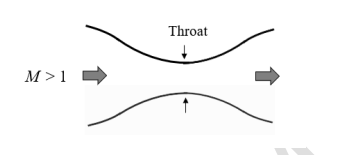
\includegraphics[width=0.5\columnwidth]{figs/Screenshot from 2025-08-23 15-45-45.png}
    \caption{Caption}
    \label{fig:placeholder}
\end{figure}

\begin{enumerate}
\begin{multicols}{2}
\item Can only be supersonic  
\item Can only be sonic  
\item Can either be sonic or supersonic  
\item Can only be subsonic  
\end{multicols}
\end{enumerate}
\hfill(GATE AE 2024)

\item Consider steady, incompressible, inviscid flow past two airfoils. The coefficient of pressure at the trailing edge of the finite angle airfoil (I) is $C_{P_I}$ and at the cusp airfoil (II) is $C_{P_{II}}$. Which one is true?  

\begin{figure}[H]
    \centering
    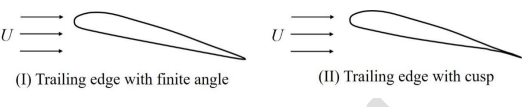
\includegraphics[width=0.5\columnwidth]{figs/Screenshot from 2025-08-23 15-54-40.png}
    \caption{Caption}
    \label{fig:placeholder}
\end{figure}

\begin{enumerate}
\item $C_{P_I} < 1,\; C_{P_{II}} < 1$  
\item $C_{P_I} = 1,\; C_{P_{II}} = 1$  
\item $C_{P_I} = 1,\; C_{P_{II}} < 1$  
\item $C_{P_I} < 1,\; C_{P_{II}} = 1$  
\end{enumerate}
\hfill(GATE AE 2024)

\item Which of the following options is/are correct?  

\begin{enumerate}
\item The stress-strain graph for a nonlinear elastic material is as shown in the figure  

\begin{figure}[H]
    \centering
    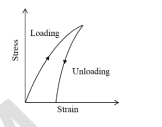
\includegraphics[width=0.5\columnwidth]{figs/Screenshot from 2025-08-23 15-55-50.png}
    \caption{Caption}
    \label{fig:placeholder}
\end{figure}

\item Material properties are independent of position in a homogeneous material  
\item An isotropic material has infinitely many planes of material symmetry  
\item The stress-strain graph for a linear elastic material is as shown in the figure  

\begin{figure}[H]
    \centering
    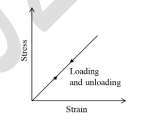
\includegraphics[width=0.5\columnwidth]{figs/Screenshot from 2025-08-23 15-56-46.png}
    \caption{Caption}
    \label{fig:placeholder}
\end{figure}

\end{enumerate}
\hfill(GATE AE 2024)

\item Which of the following statements is/are correct about a satellite moving in a geostationary orbit?  

\begin{enumerate}
\begin{multicols}{2}
\item The orbit lies in the equatorial plane  
\item The orbit is circular about the center of the Earth  
\item The time period of motion is 90 minutes  
\item The satellite is visible from all parts of the Earth  
\end{multicols}
\end{enumerate}
\hfill(GATE AE 2024)

\item In a conventional configuration airplane, the rudder can be used:  

\begin{enumerate}
\begin{multicols}{2}
\item to overcome adverse yaw during a turning maneuver  
\item to overcome yawing moment due to failure of one engine in a multi-engine airplane  
\item for landing the airplane in crosswind conditions  
\item for enhancing longitudinal stability  
\end{multicols}
\end{enumerate}
\hfill(GATE AE 2024)

\item Which of the following statements about a general aviation aircraft, while operating at point Q in the V-n diagram, is/are true?  

\begin{figure}[H]
    \centering
    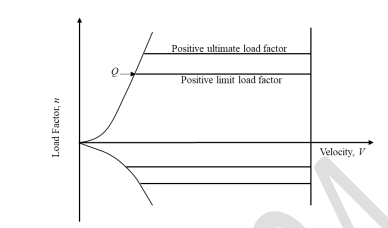
\includegraphics[width=0.5\columnwidth]{figs/Screenshot from 2025-08-23 15-58-24.png}
    \caption{Caption}
    \label{fig:placeholder}
\end{figure}

\begin{enumerate}
\begin{multicols}{2}
\item The aircraft has the highest turn rate  
\item The aircraft has the smallest turn radius  
\item The aircraft is flying with minimum drag  
\item The aircraft is operating at $C_{L,\max}$  
\end{multicols}
\end{enumerate}
\hfill(GATE AE 2024)

\item Two fair dice are rolled together. The probability of getting odd numbers on both dice is \dots (rounded off to 2 decimal places).  
\hfill(GATE AE 2024)

\item A particle acted upon by a constant force $\vec{F} = 4\hat{i} + \hat{j} - 3\hat{k}$ N is displaced from point $A(1,2,3)$ m to point $B(5,4,1)$ m. The work done by this force is \dots J (answer in integer).  
\hfill(GATE AE 2024)

\item Using Trapezoidal rule with one interval, the approximate value of $\int_1^2 \dfrac{dx}{1+x^2}$ = \dots (rounded off to 2 decimal places).  
\hfill(GATE AE 2024)

\item A material has Poisson's ratio $\nu = 0.5$ and Young's modulus $E = 2500$ MPa. The percentage change in its volume when subjected to hydrostatic stress of magnitude $10$ MPa is \dots (answer in integer).  
\hfill(GATE AE 2024)

\item An airplane experiences a net vertical ground reaction of $15000$ N during landing. The weight of the airplane is $10000$ N. The landing vertical load factor, defined as the ratio of inertial load to the weight, is \dots (rounded off to 1 decimal place).  
\hfill(GATE AE 2024)

\item An aircraft with a turbojet engine is flying at $250$ m/s. The air density is $1$ kg/m$^3$, inlet area = $1$ m$^2$, exhaust velocity relative to aircraft = $550$ m/s. Neglect pressure thrust and fuel-air ratio. The uninstalled thrust is \dots N (rounded off to nearest integer).  
\hfill(GATE AE 2024)

\item Using thin airfoil theory, the lift coefficient of a NACA 0012 airfoil at $5^\degree$ angle of attack is \dots (rounded off to 2 decimal places).  
\hfill(GATE AE 2024)

\textbf{Q.36 - Q.65 Carry TWO mark Each}

\item Given $y = e^{px}\sin(qx)$, where $p,q$ are non-zero reals, the value of  
$\dfrac{d^2y}{dx^2} - 2p\dfrac{dy}{dx} + (p^2+q^2)y$ is  
\begin{enumerate}
\begin{multicols}{4}
\item 0  
\item 1  
\item $p^2+q^2$  
\item $pq$  
\end{multicols}
\end{enumerate}
\hfill(GATE AE 2024)

\item The volume of the solid formed by a complete rotation of the shaded portion of the circle of radius $R$ about the $y$-axis is $k\pi R^3$. The value of $k$ is  
\begin{figure}[H]
    \centering
    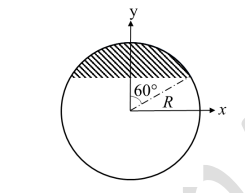
\includegraphics[width=0.5\columnwidth]{figs/Screenshot 2025-08-24 055943.png}
    \caption{Caption}
    \label{fig:placeholder}
\end{figure}
\begin{enumerate}
\begin{multicols}{4}
\item $\dfrac{5}{12}$  
\item $\dfrac{5}{24}$  
\item $\dfrac{7}{12}$  
\item $\dfrac{7}{24}$  
\end{multicols}
\end{enumerate}
\hfill(GATE AE 2024)

\item As per the International Standard Atmosphere model, which one of the following options about density variation with increase in altitude in the isothermal layer is correct?  
\begin{enumerate}
\begin{multicols}{2}
\item remains constant  
\item increases linearly  
\item decreases linearly  
\item decreases exponentially  
\end{multicols}
\end{enumerate}
\hfill(GATE AE 2024)


\item At a point in the trajectory of an unpowered space vehicle moving about the Earth, the altitude above the mean sea level is $600 \, \text{km}$, and the speed with reference to a coordinate system fixed to the center of mass of the Earth is $9 \, \text{km/s}$. Assume that the Earth is a sphere with a radius $6400 \, \text{km}$ and $GM_{\text{Earth}} = 3.98 \times 10^{14} \, \text{m}^3/\text{s}^2$. The trajectory is: 
\begin{enumerate}
\begin{multicols}{2}
\item Circular  
\item Elliptic  
\item Parabolic  
\item Hyperbolic  
\end{multicols}
\end{enumerate}
\hfill(GATE AE 2024)

\item A multistage axial compressor, with overall isentropic efficiency of $0.83$, is used to compress air at a stagnation temperature of $300 \, \text{K}$ through a pressure ratio of $10{:}1$. Each stage of the compressor is similar, and the stagnation temperature rise across each compressor stage is $20 \, \text{K}$. Assume $C_p = 1005 \, \text{J/kg.K}$ and $\gamma = 1.4$ for air. How many stages are there in the compressor?  
\begin{enumerate}
\begin{multicols}{4}
\item 17  
\item 13  
\item 19  
\item 11  
\end{multicols}
\end{enumerate}
\hfill(GATE AE 2024)

\item An aircraft with a turbojet engine is flying at $250 \, \text{m/s}$. The uninstalled thrust produced by the engine is $60000 \, \text{N}$. The heating value of the fuel is $44 \times 10^6 \, \text{J/kg}$. The engine has a thermal efficiency of $35\%$ while burning the fuel at a rate of $3 \, \text{kg/s}$. Assume the engine exit pressure to be equal to the ambient pressure. What is the propulsion efficiency of the engine under these conditions (in percentage)?  
\begin{enumerate}
\begin{multicols}{4}
\item 32.5  
\item 35.0  
\item 11.4  
\item 92.4  
\end{multicols}
\end{enumerate}
\hfill(GATE AE 2024)


\item Consider a flat plate, with a sharp leading edge, placed in a uniform flow of speed $U$. The direction of the free-stream flow is aligned with the plate. Assume that the flow is steady, incompressible and laminar. The thickness of the boundary layer at a fixed stream-wise location $L$ from the leading edge of the plate is $\delta$. Which one of the following correctly describes the variation of $\delta$ with $U$?  
\begin{enumerate}
\begin{multicols}{2}
\item $\delta \propto U$  
\item $\delta \propto U^{3/2}$  
\item $\delta \propto U^{1/2}$  
\item $\delta \propto U^{-1/2}$
\end{multicols}
\end{enumerate}
\hfill(GATE AE 2024)


\item Shock structures for flow at three different Mach numbers over a given wedge are shown in the figure below. Assuming that only the weak shock solutions are possible for the attached oblique shocks, which one of the following options is TRUE?  
\begin{figure}[H]
    \centering
    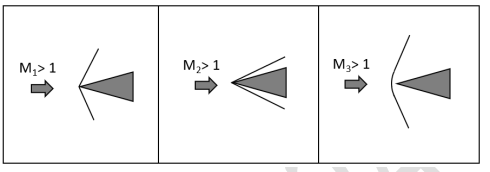
\includegraphics[width=0.5\columnwidth]{figs/Screenshot 2025-08-24 060230.png}
    \caption{Caption}
    \label{fig:placeholder}
\end{figure}
\begin{enumerate}
\begin{multicols}{2}
\item $M_1 < M_2 < M_3$  
\item $M_1 > M_2 > M_3$  
\item $M_1 < M_3 < M_2$  
\item $M_3 < M_1 < M_2$ 
\end{multicols}
\end{enumerate}
\hfill(GATE AE 2024)


\item Air flowing at Mach number $M = 2$ from left to right accelerates to $M = 3$ across an expansion corner as shown in the figure. What is the value of $\delta$ (the angle between the Forward and Rearward Mach lines) in degrees? The values of the Prandtl-Meyer functions are $\nu(3) = 49.76^\degree$ and $\nu(2) = 26.38^\degree$.  
\begin{figure}[H]
    \centering
    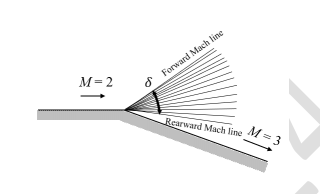
\includegraphics[width=0.5\columnwidth]{figs/Screenshot 2025-08-24 060809.png}
    \caption{Caption}
    \label{fig:placeholder}
\end{figure}
\begin{enumerate}
\begin{multicols}{4}
\item 23.38  
\item 19.47  
\item 53.38  
\item 33.91  
\end{multicols}
\end{enumerate}
\hfill(GATE AE 2024)

\item Consider the function  
$
f(x) =
\begin{cases}
x^2, & x < 0 \\
x, & x \ge 0
\end{cases}
$
where $x$ is real. Which of the following statements is/are correct?  
\begin{enumerate}
\item The function is continuous for all $x$  
\item The derivative of the function is discontinuous at $x = 0$  
\item The derivative of the function is continuous at $x = 1$  
\item The function is discontinuous at $x = 0$  
\end{enumerate}
\hfill(GATE AE 2024)

\item The figure shows plots of two yield loci for an isotropic material, where $\sigma_I$ and $\sigma_{II}$ are the principal stresses, and $\sigma_Y$ is the yield stress in uniaxial tension. Which of the following statements is/are correct?
\begin{figure}[H]
    \centering
    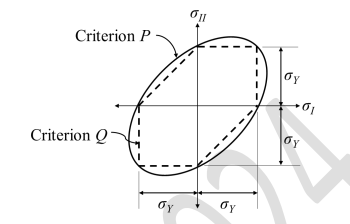
\includegraphics[width=0.5\columnwidth]{figs/Screenshot 2025-08-24 061903.png}
    \caption{Caption}
    \label{fig:placeholder}
\end{figure}
\begin{enumerate}
    \item Criterion P represents the von Mises criterion
    \item Criterion Q represents the Tresca criterion
    \item Criterion P represents the Tresca criterion
    \item Criterion Q represents the von Mises criterion
\end{enumerate}
\hfill(GATE AE 2024)

\item Which of the following statements about absolute ceiling and service ceiling for a piston-propeller aircraft is/are correct?
\begin{enumerate}
    \item The altitude corresponding to absolute ceiling is higher than that for service ceiling
    \item At the absolute ceiling, the power required for cruise equals the maximum power available
    \item The altitude corresponding to absolute ceiling is lower than that for service ceiling
    \item At the service ceiling, the maximum rate of climb is $50$ ft/min
\end{enumerate}
\hfill(GATE AE 2024)

\item For an airplane having directional / weathercock static stability, which of the following options is/are correct?
\begin{enumerate}
    \item The airplane when disturbed in yaw, from an equilibrium state, will experience a restoring moment
    \item The variation of yawing moment coefficient ($C_n$) with sideslip angle ($\beta$) for the airplane will look like 
    \begin{figure}[H]
        \centering
        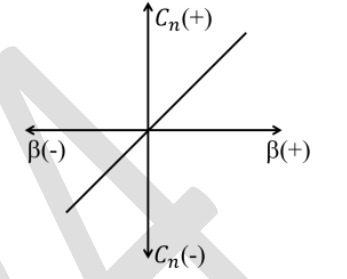
\includegraphics[width=0.5\columnwidth]{figs/Screenshot 2025-08-24 062341.png}
        \caption{Caption}
        \label{fig:placeholder}
    \end{figure}
    \item The airplane will always tend to point into the relative wind
    \item The airplane when disturbed in yaw will return to equilibrium state in a finite amount of time after removing the disturbance
\end{enumerate}
\hfill(GATE AE 2024)

\item Which of the following statements is/are TRUE for an axial turbine?
\begin{enumerate}
    \item For a fixed rotational speed, the mass flow rate increases with increase in the flow coefficient
    \item The absolute stagnation enthalpy of the flow decreases across the nozzle row
    \item The relative stagnation enthalpy remains unchanged through the rotor
    \item For a fixed rotational speed, the mass flow rate remains unchanged with a change in the flow coefficient
\end{enumerate}
\hfill(GATE AE 2024)

\item Which of the following statements is/are TRUE for a single stage axial compressor?
\begin{enumerate}
    \item Starting from design condition and keeping the mass flow rate constant, if the blade RPM is increased, the compressor rotor may experience positive incidence flow separation (actual relative flow angle greater than the design blade angle)
    \item Starting from design condition at the same blade RPM, if the mass flow rate is increased, the compressor rotor may experience positive incidence flow separation (actual relative flow angle greater than the design blade angle)
    \item Keeping the mass flow rate constant, if the blade RPM is increased, the compressor may experience surge
    \item At the same blade RPM, if the mass flow rate is increased, the compressor may experience surge
\end{enumerate}
\hfill(GATE AE 2024)

\item Consider the matrix $A = \myvec{ 5 & -4 \\ k & -1 }$, where $k$ is a constant. If the determinant of $A$ is $3$, then the ratio of the largest eigenvalue of $A$ to the constant $k$ is \dots (rounded off to $1$ decimal place).
\hfill(GATE AE 2024)

\item The state of stress at a point is caused by two separate loading cases. One of them produces a pure uniaxial tension along the $x'$ direction, and other one produces a pure uniaxial compression along the $y'$ direction. The sum of maximum and minimum principal stresses for the resultant state of stress caused by both loads acting simultaneously is \dots N/mm$^2$ (rounded off to $1$ decimal place).
\begin{figure}[H]
    \centering
    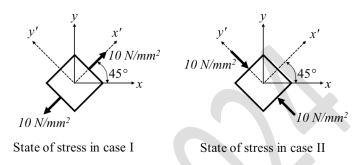
\includegraphics[width=0.5\columnwidth]{figs/Screenshot 2025-08-24 062517.png}
    \caption{Caption}
    \label{fig:placeholder}
\end{figure}
\hfill(GATE AE 2024)

\item In the figure shown below, the magnitude of internal force in member BC is \dots N (rounded off to $1$ decimal place).
\begin{figure}[H]
    \centering
    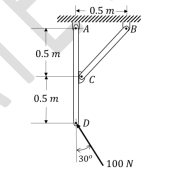
\includegraphics[width=0.5\columnwidth]{figs/Screenshot 2025-08-24 062627.png}
    \caption{Caption}
    \label{fig:placeholder}
\end{figure}
\hfill(GATE AE 2024)

\item The cross section of a thin-walled beam with uniform wall thickness $t$, shown in the figure, is subjected to a bending moment $M_x = 10$ Nm. If $h = 1$ m and $t = 0.001$ m, the magnitude of maximum normal stress in the cross section is \dots N/m$^2$ (answer in integer).

\begin{figure}[H]
    \centering
    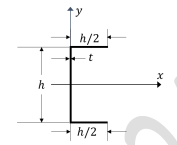
\includegraphics[width=0.5\columnwidth]{figs/Screenshot 2025-08-24 062733.png}
    \caption{Caption}
    \label{fig:placeholder}
\end{figure}
\hfill(GATE AE 2024)

\item The equations of motion for a two degrees of freedom undamped spring-mass system are:
$
m \ddot{x}_1 + 2k x_1 - k x_2 = 0
$
$
m \ddot{x}_2 - k x_1 + 2k x_2 = 0
$
where $m$ and $k$ represent mass and stiffness respectively, in corresponding SI units, and $x_1$ and $x_2$ are the degrees of freedom. The larger of the two natural frequencies is given by: $\omega = \alpha \sqrt{\frac{k}{m}}$ rad/s. The value of $\alpha$ is \dots (rounded off to $2$ decimal places).
\hfill(GATE AE 2024)

\item Consider the plane strain field given by:
$
\varepsilon_{xx} = 10xy^2, \quad \varepsilon_{yy} = -5x^2y, \quad \gamma_{xy} = Axy(2x - y)
$
where $A$ is a constant and $\gamma_{xy}$ is the engineering shear strain. The value of the constant $A$ for the strain field to be compatible is \dots (rounded off to $1$ decimal place).
\hfill(GATE AE 2024)

\item A chemical rocket with an ideally expanded flow through the nozzle produces $5 \times 10^6$ N thrust at sea level. The specific impulse of the rocket is $200$ s and acceleration due to gravity at the sea level is $9.8$ m/s$^2$. The propellant mass flow rate out of the rocket nozzle is \dots kg/s (rounded off to the nearest integer).
\hfill(GATE AE 2024)

\item A centrifugal compressor is designed to operate with air. At the leading edge of the tip of the inducer (eye of the impeller), the blade angle is $45^\degree$, and the relative Mach number is $1.0$. The stagnation temperature of the incoming air is $300$ K. Consider $\gamma = 1.4$. Neglect pre-whirl and slip. The inducer tip speed is \dots m/s (rounded off to the nearest integer).
\hfill(GATE AE 2024)

\item Consider the following Fanno flow problem: Flow enters a constant area duct at a temperature of $273$ K and a Mach number $0.2$ and eventually reaches sonic condition (Mach number = $1$) due to friction. Assume $\gamma = 1.4$. The static temperature at the location where sonic condition is reached is \dots K (rounded off to $2$ decimal places).
\hfill(GATE AE 2024)

\item Consider an artificial satellite moving around the Moon in an elliptic orbit. The altitude of the satellite from the Moon's surface at the perigee is $25$ km and that at the apogee is $134$ km. Assume the Moon to be spherical with a radius of $1737$ km. The trajectory is considered with reference to a coordinate system fixed to the center of mass of the Moon. The ratio of the speed of the satellite at the perigee to that at the apogee is \dots (rounded off to $2$ decimal places).
\hfill(GATE AE 2024)

\item For an aircraft moving at $4$ km altitude above mean sea level at a Mach number of $0.2$, the ratio of equivalent air speed to true air speed is \dots (rounded off to $2$ decimal places). The density of air at mean sea level is $1.225$ kg/m$^3$ and at $4$ km altitude is $0.819$ kg/m$^3$.
\hfill(GATE AE 2024)

\item For a general aviation airplane, one of the complex conjugate pair of eigenvalues for longitudinal dynamics is given by $-0.039 \pm 0.0567i$ (in SI units). If the system is disturbed to excite only this mode, the time taken for the amplitude of response to become half in magnitude is \dots s (rounded off to $1$ decimal place).
\hfill(GATE AE 2024)

\item The figure (not to scale) shows a control volume to estimate the forces on the airfoil with elliptic cross-section. Surfaces 2 and 3 are streamlines. Velocity profiles are measured at the upstream end (surface 1) and at the downstream  end (surface 4) of the control volume.  The drag coefficient for the airfoil is defined as 
$
C_d = \frac{D}{\frac{1}{2} \rho U_\infty^2 c},
$
where $D$ is the drag force on the airfoil per unit span and $\rho$ is the density of the air. The static pressure, $p_\infty$, is constant over the entire surface of the control volume. Assuming the flow to be incompressible, two-dimensional and steady, the $C_d$ for the airfoil is \dots (rounded off to $3$ decimal places).

\begin{figure}[H]
    \centering
    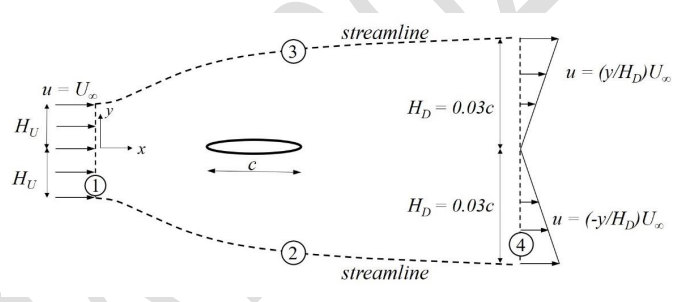
\includegraphics[width=0.5\columnwidth]{figs/Screenshot 2025-08-24 063236.png}
    \caption{Caption}
    \label{fig:placeholder}
\end{figure}
\hfill(GATE AE 2024)
 
\item An airplane of mass $1000$ kg is in a steady level flight with a speed of $50$ m/s. The wing has an elliptic planform with a span of $20$ m and planform area $31.4$ m$^2$. Assuming the density of air at that altitude to be $1$ kg/m$^3$ and acceleration due to gravity to be $10$ m/s$^2$, the induced drag on the wing is \dots N (rounded off to $1$ decimal place).
\hfill(GATE AE 2024)

\item It is desired to estimate the aerodynamic drag, $D$, on a car traveling at a speed of $30$ m/s. A one-third scale model of the car is tested in a wind-tunnel following the principles of dynamic similarity. The drag on the scaled model is measured to be $D_m$. The ratio $D/D_m$ is \dots (rounded off to $1$ decimal place).
\hfill(GATE AE 2024)

    
\end{enumerate}
\end{document}